\appendixsection{Standard methods}

\begin{appendixframe}{Physics-Informed Neural Networks}
	\labelsubappendixframe{frame:pinns}
	\textbf{Standard PINNs\footcite{RAISSI2019686} (Weak BC) :} Find the optimal weights $\theta^\star$, such that
	\begin{equation}
		\label{eq:opt_pb}
		\theta^\star = \argmin_{\theta}	\big( \omega_r \; J_r(\theta) + \omega_b \; J_b(\theta) \big),
		\tag{$\mathcal{P}_\theta$}
	\end{equation}

	\vspace{-5pt}
	with
	\vspace{5pt}

	\begin{minipage}{0.2\linewidth}
		\flushright
		\textcolor{orange}{residual loss}

		\vspace{12pt}
		\textcolor{red}{boundary loss}
	\end{minipage}
	\begin{minipage}{0.68\linewidth}
		\centering
		\fcolorbox{orange}{white}{
			$J_r(\theta) =
			\int_{\mathcal{M}}\int_{\Omega}
			\big| \mathcal{L}\big(u_\theta(\bm{x},\bm{\mu});\bm{x},\bm{\mu}\big)-f(\bm{x},\bm{\mu}) \big|^2 d\bm{x} d\bm{\mu},$}
		
		\vspace{3pt}
		\fcolorbox{red}{white}{
			$J_b(\theta) =
			\int_{\mathcal{M}}\int_{\partial \Omega} \big| u_\theta(\bm{x},\bm{\mu}) - g(\bm{x},\bm{\mu}) \big|^2 d\bm{x} d\bm{\mu},$}
	\end{minipage}
	
	\vspace{5pt}
	where $u_\theta$ is a neural network, $g=0$ is the Dirichlet BC. 

	\vspace{2pt}
	In \eqref{eq:opt_pb}, $\omega_r$ and $\omega_b$ are some weights.

	\vspace{5pt}
	\textbf{Monte-Carlo method :} Discretize the cost functions by random process.
	\vspace{15pt}
\end{appendixframe}

\begin{appendixframe}{Physics-Informed Neural Networks}[noframenumbering]
	\textbf{\textcolor{red}{Improved PINNs\footcite{LagLikFot1998,FraMicNav2024} (Strong BC)} :} Find the optimal weights $\theta^\star$ such that
	\begin{equation*}
		% \label{eq:opt_pb_nobc}
		\theta^\star = \argmin_{\theta}	\big( \omega_r \; J_r(\theta) + \Ccancel[red]{\omega_b \; J_b(\theta)} \big),%\tag{$\mathcal{P}_\theta$}
	\end{equation*}
	
	\vspace{-5pt}
	with $\omega_r=1$ and
	\vspace{5pt}

	\begin{minipage}{0.2\linewidth}
		\flushright
		\textcolor{orange}{residual loss}
	\end{minipage}
	\begin{minipage}{0.68\linewidth}
		\centering
		\fcolorbox{orange}{white}{
			$J_r(\theta) =
			\int_{\mathcal{M}}\int_{\Omega}
			\big| \mathcal{L}\big(u_\theta(\bm{x},\bm{\mu});\bm{x},\bm{\mu}\big)-f(\bm{x},\bm{\mu}) \big|^2 d\bm{x} d\bm{\mu},$}
	\end{minipage}

	\vspace{15pt}
	\begin{minipage}{0.75\linewidth}
		where $u_\theta$ is a neural network defined by
		\begin{equation*}
			\textcolor{red}{u_{\theta}(\bm{x},\bm{\mu}) = \varphi(\bm{x}) w_{\theta}(\bm{x},\bm{\mu}) + g(\bm{x},\bm{\mu}),}
		\end{equation*}
		with $\varphi$ a level-set function, $w_\theta$ a NN and $g=0$ the Dirichlet BC. 
	\end{minipage}
	\begin{minipage}{0.23\linewidth}
		\vspace{-15pt}
		\hspace{-23pt}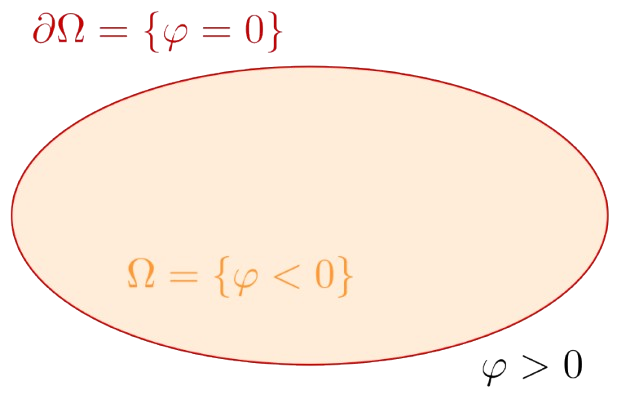
\includegraphics[width=1.3\linewidth]{images/intro/levelset.png}
	\end{minipage}

	\vspace{5pt}
	Thus, the Dirichlet BC is imposed exactly in the PINN : \textcolor{red}{$u_{\theta} = g$ on $\partial \Omega$}.

	\vspace{15pt}
\end{appendixframe}

\addtocounter{subappendixframenumber}{1}
\begin{appendixframe}{Finite Element Methods\footcite{Ern2004TheoryAP}}	
	\labelsubappendixframe{frame:fems}
	\textbf{Variational Problem :} 
	\begin{equation}
		\label{eq:weakform}
		\text{Find } u_h\in V_h^0 \;\text{such that}, \forall v_h\in V_h^0, a(u_h,v_h)=l(v_h),
		\tag{$\mathcal{P}_h$}
	\end{equation}
	\vspace{1pt}
	with $h$ the characteristic mesh size, $a$ and $l$ the bilinear and linear forms given by
	\vspace{-3pt}
	\begin{equation*}
		a(u_h,v_h)=
		\frac{1}{\text{Pe}} \int_{\Omega}D \nabla u_h \cdot  \nabla v_h+
		\int_{\Omega} R \, u_h \, v_h  +
		\int_{\Omega} v_h \, C \cdot \nabla u_h, \quad l(v_h)=\int_{\Omega} f \, v_h,
	\end{equation*}

	\begin{minipage}[t]{0.7\linewidth}
		\vspace{-3pt}
		and $V_h^0$ the finite element space defined by
		\vspace{-3pt}
		\begin{equation*}
			% \label{eq:Vh}
			V_h^0 = \left\{v_h\in C^0(\Omega),\; \forall K\in \mathcal{T}_h,\; v_h\vert_{K}\in\mathbb{P}_k,v_h\vert_{\partial\Omega}=0\right\},
		\end{equation*}
		
		\vspace{-3pt}
		where $\mathbb{P}_k$ is the space of polynomials of degree at most $k$.
		
		\vspace{10pt}
		\textbf{Linear system :} Let $(\phi_1,\dots,\phi_{N_h})$ a basis of $V_h^0$.
	\end{minipage} \qquad \begin{minipage}[t][][b]{0.2\linewidth}
		% \vspace{-5pt}
		\centering
		\pgfimage[width=0.9\linewidth]{images/intro/FEM_triangle_mesh.png}
		
		\footnotesize
		$\mathcal{T}_h = \left\{K_1,\dots,K_{N_e}\right\}$
		
		\tiny
		($N_e$ : number of elements)
	\end{minipage}
	
	\vspace{-5pt}
	Find $U\in\mathbb{R}^{N_h}$ such that \hspace{40pt} $AU=b$
	
	with 
	\begin{equation*}
		A=\big(a(\phi_i,\phi_j)\big)_{1\le i,j\le N_h} \quad \text{and} \quad b=\big(l(\phi_j)\big)_{1\le j\le N_h}.
	\end{equation*}
	\vspace{-3pt}
\end{appendixframe}

\appendixsection{More}

\begin{appendixframe}{Adaptive mesh refinement}
	\labelsubappendixframe{frame:amr}
	Use of the \textbf{Dorfler marking strategy} to refine the mesh $\mathcal{T}_h$. \citep{dorfler_1996}
	TODO
	% \begin{equation*}
    %     \eta_{res} = \left(\sum_{T\in\mathcal{T}_h}\eta_{res,T}^2\right)^{1/2}, \quad \eta_{res,T}^2 = h_T^4 \|R\|_{L^2(T)}^2 + \frac{1}{2} \sum_{E \in \partial T} h_E^2 \|J\|_{L^2(E)}^2
    % \end{equation*}
\end{appendixframe}